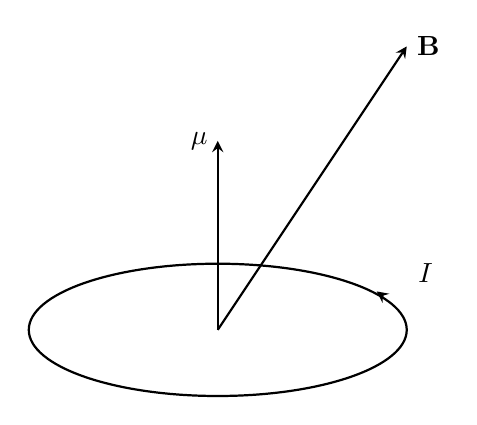
\begin{tikzpicture}[scale=1.2,>=stealth]

% --- Parte destra: Spira con corrente ---
\draw[thick] (6,0) ellipse (2cm and 0.7cm);

% Corrente I lungo ellisse (arco ellittico)
\draw[->,thick] (7.75,0.35) arc[start angle=20,end angle=25,x radius=2cm,y radius=0.7cm];
\node at (8.2,0.6) {$I$};

% Momento magnetico mu
\draw[->,thick] (6,0) -- (6,2) node[left] {$\mu$};

% Campo magnetico B
\draw[->,thick] (6,0) -- (8,3) node[right] {$\mathbf{B}$};

\end{tikzpicture}